\section{Methods Supplemental Information}


\subsection{Experimental Procedures}

\subsubsection{Test Case Sequences}


Throughout the experimental campaign, we performed the following test case sequences. The test cases are presented below with our internal naming scheme that begins with a three digit number that represent the nominal values for the HVOF process inputs. The first digit represents the total mass flow (5 = 13.0 g/s), the second digit represents the equivalence ratio (1 = 0.6, 3 = 0.8), and the third digit represents the potassium mass fraction (3 = 0.1\% and 6 = 1.0\%). A 'x' indicates that the nominal value was varied during that sequence. The sequence is then appended with 'pos' or 'pow' to indicate a position or power sweep, respectively. The absence of 'pos' or 'pow' indicates that the SFR-maximized position of 180mm downstream of the barrel exit and full laser power (7 mJ) were used. A given test case sequence is appended with a 'run number' to indicate repeats of the sequence performed on the same day. 


\begin{itemize}
    \item 536 Position: Varying motorized stage position. Full laser power. Kwt = 1\%, phi = 0.8 (presented in main text). Performed on 2023-04-07, 2023-05-12, 2023-05-18.
    \item 516 Position: Varying motorized stage position. Full laser power. Kwt = 1\%, phi = 0.6 (presented in main text). Performed on 2023-05-24.
    \item 53x: Varying potassium mass fraction. motorized stage at nominal position. Full laser power. (presented in main text). Performed on each date. 
    \item 536 Power: Varying laser power. motorized stage at nominal position. Kwt = 1\%. Performed on each date. 
    \item 5xx: Varying potassium mass fraction and equivalence ratio. motorized stage at nominal position. Full laser power. Performed on 2023-05-24.
    \item 5x6\_pos/5x3\_pos: Varying motorized stage position and equivalence ratio. Full laser power. Kwt = 0.1\% or 1\%. Performed on 2023-05-24.
\end{itemize}

For each diagnostic, data is obtained continuously throughout the experiment and indexed in time. For each individual test case, there are a number of repeated acquisitions depending on the duration of the test case and acquisition rate of the diagnostic. In the data processing, these repeated acquisitions are averaged to obtain a single value for each test case before further analysis (e.g. fitting). For statistics across runs presented in the main text, the variation within repeat acquisitions is not considered. 

The syringe pump limits the duration of a given test case sequence, with shorter durations at high potassium mass fraction. Furthermore, it was not possible to maintain consistent durations for the same test cases performed in different sequences.
The time limitation on seeding duration limits the AES diagnostic more than the MWS diagnostic. The AES diagnostic must wait 1 second between LED switching events to allow for the LED to stabilize. Additionally, the multiplexer switches every 10s. Therefore a minimum of at least 20 s is needed for a nK measurement at both location, but ideally multiple measurements are taken at each location to ensure reproducibility. The MWS diagnostic, on the other hand, is continuously acquiring at the repetition rate of the laser (5-12 Hz).  Therefore for a given test case sequences, the MWS diagnostic has more data than the AES diagnostic. For the standard test case sequences outlined above, approximately 1 minute was used for each test case and data is presented for both diagnostics.




\subsubsection{Experiment Overviews}

Below are overviews of the experiments performed. The independent variables that were varied throughout the experiments are shown and the colored regions are test case sequences. Times are in PST. Note that not all test case sequences that were performed were analyzed in the main text. 


\foreach \date in {2023-04-07, 2023-05-12, 2023-05-18, 2023-05-24}{
    \begin{figure}[h]
        \centering
        \includegraphics[width=0.9\linewidth]{\repodir/experiment/analysis/auto/output/figures/tc_plot_\date.png} 
        \caption{Experiment Overview for \date. The colored regions are test case sequences.}
        \label{fig:SI_expt_overview_\date}
    \end{figure}

    \begin{figure}[h]
        \centering
        \includegraphics[width=0.9\linewidth]{\repodir/experiment/analysis/auto/output/figures/other_signals/tc_plot_\date.png} 
        \caption{Additional signals for \date. The colored regions are test case sequences with the same scheme as as in \ref{fig:SI_expt_overview_\date}.}
        \label{fig:SI_expt_overview_other_\date}
    \end{figure}

}

\clearpage

\subsection{Data Pipeline}

The results of this work are created from a set of codes located at \url{https://github.com/MHDLab-Projects/MHD-Photoionization}. The final results and figures are the output of a data pipeline.  The data pipeline starts from the raw experimental dataset, which consists of unprocessed data taken during the experiments. The data pipeline consists of a series of shell scripts that in turn primarily run python scripts. Therefore, the shell scripts in the repository can act as a map of the data processing methodology. The data pipeline has the following steps: 

\begin{enumerate}
    \item Data Munging (\texttt{/automation/munge.sh}): The raw data is initially processed to reduce the size of the dataset and to convert the data to common formats of either 'tdms' (National Instruments) or 'cdf' (xarray python package). This includes the standard data processing steps of our lab for time series data (located in /PostProcessor), notably resampling from 1kHz data acquisition rate to a 1 sample per second. Additionally, resampling and combining of individual acquisition files is done for the MWS oscilloscope data.  At this stage, each experiment date is processed separately.
    \item Process Munged Data (\texttt{/automation/process\_munged.sh}): Data is combined from different dates to create single datasets for each diagnostic. Then, test case time windows are used create datasets for the test case sequences, with the independent variables (Potassium mass fraction, equivalence ratio, stage position, laser power, experiment date, run number, acquisition number) being added as coordinates in xarray datasets.
    \item Create Final Dataset (\texttt{/automation/final\_dataset.sh}): The final dataset is created by applying various analysis steps (data extraction, fitting, etc.) to the processed data. 
    \item Generate Figure Panels (\texttt{/automation/gen\_fig\_panels.sh}): The final dataset is used to generate the figure panels (A, B, C, etc.)for the main manuscript. 
    \item Render Figures (\texttt{/automation/render\_figures.sh}): The figure panels are combined into the final figures for the manuscript. The figures panels are laid out in SVG files, and the SVG file is rendered with Inkscape to create the final figure PNG file. 
\end{enumerate}

In addition to the above steps that lead to the final figures, the repository contains a variety of analysis scripts that contains supplemental/exploratory figures that were generated throughout the data analysis process. These scripts are rendered as jupyter notebooks in a subfolder called 'nb\_render', relative to the analysis script. These notebooks are collected and rendered to PDFs in final/output/nb\_renders. 

The supplemental analysis scripts need to be run to generate the supplemental figures. The shell commands \texttt{automation/render\_all\_expt.sh} and \texttt{automation/render\_all\_expt.sh final} will render these scripts to Jupyter notebooks 'renders'. During this process many of the supplemental figures are created, though those figures could also be generated running the scripts directly. Finally, there are scripts not automated in the above process that contain some supplemental figures, which are outlined in \texttt{automation/supp\_scripts.sh}. 

\clearpage
\subsection{Microwave Scattering (MWS) }


\subsubsection{Setup Description}
\begin{figure}[]
\centering
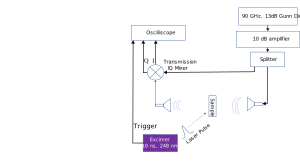
\includegraphics[width=0.8\textwidth]{\repodir/final/figures/SI/output/MWS_Setup.png}
\caption{Microwave scattering setup. Left: An image of the setup. Right: A schematic of the setup. LO: local oscillator. I: In-phase Q: Quadrature.  }
\label{fig:SI_MWS_Setup}
\end{figure}

The microwave scattering setup is shown in Figure \ref{fig:SI_MWS_Setup}. The parts were ordered from Erevant, formerly Sage Millimeter. The system is W-band and based on WR-10 waveguides. The microwave source is a 90 GHz Gunn oscillator (SOM-90305213-10-S1) with an output power of +13 dBm. The output of this source is fed into a 10 dB gain, +15 dBm P1dB, in-line waveguide power amplifier (SBP-7531141015-1010-E1). The output of the power amplifier is then fed into a 4-way in-line power divider (SWP-90310404-10-E1). In the current configuration, only two outputs of the power divider are used, and the remaining two are terminated with waveguide terminators (SWL-1027-S1). One power of the power divider is used for the main transmitted power, which is sent through waveguides to a rectangular horn antenna (SAR=2013-10-S2) that transmits the microwaves into free space. The transmitted microwaves after the sample are collected by the same type of horn, and the collected microwaves are sent to the IQ mixer (SFQ-75311415-1010SF-N1-M). The LO input of the IQ mixer is fed by the remaining port of the power divider. 

% Between the power divider and the LO input there is a phase shifter (STP-18-10-M2) that is typically used to maximize the I signal in the absence of a sample. 

The I and Q signals from the oscilloscope are fed directly into a Teledyne Leroy WavePro 404HD-MS Oscilloscope.  The oscilloscope is triggered from the excimer laser. 

The oscilloscope was used with a 1 MOhm input impedance with DC coupling for the I/Q signals, and 50 ohm input impedance for the photodiode signals. The vertical coupling was 20mV per division on 2023-04-07 and 2023-05-12, and 50mV per division on 2023-05-18 and 2023-05-24 for the IQ signals. There is was an increased signal intensity on the second two dates, which we suspect was due to cleaning of residue from the microwave horns, as discussed below. The vertical coupling of the photodiode signals was 20 mV/division for on-peak, and 10mV per division off-peak. The horizontal coupling was 10 $\mu s$ per division. 

The excimer laser was used with 12 kV pulse power. The repetition rate of the laser varied: 2023-04-07 5Hz, 2023-05-12: 12 Hz, 2023-05-18: 5 Hz, 2023-05-24: 5 Hz. The oscilloscope was used with no averaging of acquisitions, with a file saved for each acquisition. The repetition rate was limited by the rate at which the oscilloscope could save individual files to disk. 

The excimer laser is sent through a 90/10 UV beam splitter with the 10 \% sent to a photovoltaic power meter (Ophir PD-10C). There is an iris with a 2.7 \pm 0.05 mm opening before a UV enhanced neutral density filter with optical density of 3 before the power meter. The power data was not used in this analysis but is present in the dataset. The remaining 90 \% of the laser is directed through a Thorlabs FW 102C Filter Wheel. The filter wheel housed Thorlabs reflective UV neutral density filters. These neutral density filters have been observed to degrade from continued use with the excimer laser, and the laser power was measured before an after the experiment to ensure there was no significant degradation in filter performance. After the filter wheel, the laser is redirected with a UV mirror (Acton Instruments, 248-FR45-ID-MB) to the center of the microwave horns. Everything including the final mirror is located on the motorized stage, which moves parallel to the torch axis.  

The distance between the horns is 85.725 mm. The mirror that sends the excimer beam to the measurement location is located 247 mm downstream along the torch axis, 397 mm horizontally (along the table) perpendicular from the torch axis, and 65 mm vertically above the torch axis. 


\subsubsection{Data Processing and Fitting}

The raw MWS data consists of individual files containing channel time traces and each raw data file corresponds to to an individual laser pulse. No averaging of multiple laser pulses occurs before the data is saved to disk. While the data is writing to disk, laser pulses can be missed. After 2023-05-12,  the reptation rate was maximized to 5 Hz to minimize this effect. 

The MWS data is first munged by combining all individual acquisitions files into a single dataset with a common oscilloscope time axis. To reduce the size and processing time of this dataset the data is resampled. Within the region 0f 700 to 1500 ns (the laser pulse is at approximately 800 ns, see Figure 2 in the main text) the data is resampled by grouping datapoints into groups of 10 averaging. Outside of this region the data is grouped into 1000 datapoints and averaged. The effect of this resampling can be seen in \ref{fig:SI_mws_resampling}

\begin{figure}
\centering
\includegraphics[width=0.8\textwidth]{\repodir/experiment/analysis/mws/resampling/output/figures/mws_sample_nors_compare.png}
\caption{Comparison of the resampling methods. Both left and right panels show the same time trace, with the right panel being zoomed into the peak.}
\label{fig:SI_mws_resampling}
\end{figure}

\ref{fig:SI_mws_processing_overview} shows the following processing steps for the MWS data to determine the AS profiles as described in the text.

The fit preparation pipeline consists of the following steps:

\begin{enumerate}
    \item The data is interpolated to a grid with 0.01 $\mu s$ spacing.
    \item the data is resampled, averaging groups of 10 datapoints to a grid with 0.1 $\mu s$ spacing.
    \item  All AS data with a maximum AS value less than $5e-4$ are removed.
    \item the AS data is normalized to the maximum AS value.
    \item Any data with an absolute value of the AS in either of the time windows 40 to 50 $\mu s$ after the laser pulse or 20 to 50 $\mu s$ after the laser pulse is removed. This is to remove acquisitions with large AS spike that occurs in the absence of a laser. 
\end{enumerate}


For the exponential fit the data is down selected to a window of 5 to 15 $\mu s$ after the laser pulse and fit with an exponential fit model $y = A \exp(-t/\tau) $.


\begin{figure}[]
\centering
\includegraphics[width=0.8\textwidth]{\repodir/experiment/analysis/mws/output/figures/mws_processing_overview.png}
\caption{Microwave processing overview. From top to bottom: A) raw I and Q signals. B) the calculated magnitude C) The absolute Transmission. D) Absolute AS. See main text for formulas.  }
\label{fig:SI_mws_processing_overview}
\end{figure}


\subsubsection{No Torch Measurements}

On each date, the microwave transmission magnitude with nothing in between the horns, $U_{nothing}$, was measured. During these measurements all other settings the same (excimer laser, oscilloscope, etc.) compared to the main experimental measurements, except that the oscilloscope time window may be 250 $\mu s$ used for the Silicon measurements may have been used. An example measurement of $U_{nothing}$ is shown in \ref{fig:SI_MWS_nothing_time_trace}. For approximately 1 $\mu s$ there is electronic interference from the laser pulsing, which also appears in the main experimental transmission measurements. 



\begin{figure}[]
\centering
\includegraphics[width=0.8\textwidth]{\repodir/final/dataset/output/figures/mws_nothing_time_trace_2023-05-18.png}
\caption{Time trace from 2023-05-18 of the transmission measurement without any free jet.}
\label{fig:SI_MWS_nothing_time_trace}
\end{figure}

On 2023-05-24 the transmission was measured as a function of position as shown in \ref{fig:SI_MWS_nothing_motor}. There is a slight increase in transmission when the stage is moved as close as possible to the barrel exit, possibly due to reflections from the barrel.


\begin{figure}
\centering
\includegraphics[width=0.8\textwidth]{\repodir/final/dataset/output/figures/mws_nothing_motor_2023-05-24.png}
\caption{Motorized stage for position dependent transmission measurements.}
\label{fig:SI_MWS_nothing_motor}
\end{figure}


The  measured at the nominal position (180 mm) for each of the dates is presented in \ref{fig:SI_MWS_nothing_T0}A. Note that for 2023-05-12, the measurement was only taken at the barrel exit, which is corrected by a factor of 0.95 to estimate the transmission at the nominal position. This factor is determined from the ratio of the transmission at the nominal position to the transmission at the barrel exit from figure \ref{fig:SI_MWS_nothing_motor}. On 2023-05-18, a blue residue/corrosion was found in the waveguides, possibly from a chemical reaction or deposition from the seeded free jet. The microwave horns were cleaned and other waveguide parts were replaced. This change could explain the increased absolute transmission on 2023-05-18 and 2023-05-24.  

\ref{fig:SI_MWS_nothing_T0}B shows the absolute transmission of the magnitude before the laser pulse for the case 536\_pos, for different dates. The transmission is then measured with the sample in place. The transmission is then calculated as the ratio of the sample transmission to the transmission with nothing in place. An example of this is shown in \ref{fig:SI_MWS_nothing_T0}.  


\begin{figure}[]
\centering
\includegraphics[width=0.8\textwidth]{\repodir/final/analysis/mws/output/figures/mws_nothing_T0.png}
\caption{A) Measurement of transmission without any torch at a position of 180 mm (except 2023-05-12, as described elsewhere in SI) B) position dependent transmission measurement.}
\label{fig:SI_MWS_nothing_T0}
\end{figure}

\subsubsection{Silicon test sample}

Before each experiment we performed measurements with a silicon sample in the location of the torch to ensure the system was functioning properly. 

The silicon wafer was ordered from MTI corporation (Item Number: SIUa50D05C1R1000) and has the properties shown in Table \ref{table:material_properties}.

\begin{table}[h]
\centering
\begin{tabular}{|l|l|}
\hline
Property & Value \\
\hline
Single crystal & Si \\
Conductive type & N type, undoped \\
Resistivity & > 1000 ohm-cm \\
Size & 2" diameter x 0.5 mm \\
Orientation & (100) \\
Polish & one side polished \\
Surface roughness & < 5A RMS \\
\hline
\end{tabular}
\caption{Properties of the test silicon wafer}
\label{table:material_properties}
\end{table}

The silicon measurements are shown in \ref{fig:SI_MWS_Silicon}. The measured exponential time constant is consistent with the minority carrier lifetime in an undoped silicon wafer. \cite{tyagiMINORITYCARRIERRECOMBINATION, delalamoModellingMinoritycarrierTransport1987} 

\begin{figure}[]
\centering
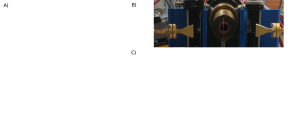
\includegraphics[width=0.8\textwidth]{\repodir/final/figures/SI/output/MWS_Silicon.png}
\caption{Measurements of the MWS system with a Silicon sample. A) Power dependent measurements of I, Q, and the calculated magnitude $U$. B) a picture of the silicon sample placed in the location of the torch. C) the $\Delta AS$ curve for the silicon sample with an exponential fit. }
\label{fig:SI_MWS_Silicon}
\end{figure}








\clearpage
\subsubsection{Laser Profile and Power}

The laser profile was measured by imaging the laser beam on a white beam block. The images were taken with a Thorlabs DCC1240C-HQ camera, and are shown in \ref{fig:SI_Laser_Profile}A. Cross sections of this image are taken to obtain the full width at half maximum (FWHM) of the laser profile and calculate the area of the beam.  

\begin{figure}[H]
\centering
\includegraphics[width=0.8\textwidth]{\repodir/experiment/analysis/mws/output/figures/laser_profile.png}
\caption{Laser profile measurement. A) The image of the laser profile. B) The cross sections of the laser profile. The width of the cross sections and calculated area are indicated in the figure.}
\label{fig:SI_Laser_Profile}
\end{figure}

The laser power was measured with an Ophir PE25BG-C Pyroelectric power meter before and after the experiments as shown in \ref{fig:SI_Laser_Energy} 



\begin{figure}[H]
\centering
\includegraphics[width=0.8\textwidth]{\repodir/experiment/analysis/various/output/figures/laser_energy_date.png}
\caption{Measurement of the laser pulse energy. The datapoints include measurements before and after the experiment. The average laser power across all measurements is shown in the figure title. }
\label{fig:SI_Laser_Energy}
\end{figure}


\clearpage
\subsection{Absorption Emission Spectroscopy (AES) Setup}

\subsubsection{Setup Description}

The LED is a Thorlabs M780F2 780 nm LED. The LED is driven by a Thorlabs T-Cube LED Driver. With input current set to approximately 0.6 A. The LED is fed into a Thorlabs M28L02 fiber with 400 $\mu m$ diameter and 0.39 NA. The fiber is then connected to the input of a  Ocean Optics MPM-2000-UV-VIS600-2X8 Multiplexer.  The multiplexer can send light to either of the AES diagnostics (barrel exit and MWS measurement location). The multiplexer continuously switches between the locations every 10 seconds throughout the duration of the measurement. After collection of light with the collection lenses (described below), the light of both barrel exit and mobile setup is sent back to the multiplexer. Finally, the light passes from multiplexer to spectrometer through an Ocean Optics QP-600-2-VIS-NIR fiber.

Because both AES diagnostics were multiplexed to the same spectrometer, one AES measurement could be taken at a time. Throughout the measurement the multiplexer switched continuously between the two AES diagnostics, so the measurements at the two AES locations are not simultaneous.

For the barrel exit measurement, the light is collimated with a RC02SMA-P01 reflective parabolic mirror. The light is directed at a 90 degree angle with a MRA05-E3 dielectric mirror. The light passes through a glass slide which is used to protect the optics from the torch. The collecting side uses the same glass slide and parabolic mirror. The light is collected with a RC04-SMA-P01 parabolic mirror. There are irises of approximately 1 mm on the sending and collecting sides. The light is sent from the multiplexer to the collimating lens with a Thorlabs M38L02 200um 0.39 NA fiber, and sent from the collection lens to the multiplexer with a Thorlabs M53L02 600 um 0.5NA fiber. The beam is positioned to go through the center of the torch at approximately 1/8 inch \pm 1/16 inch downstream of the barrel exit. The beam diameter is approximately 3/32 inch to 4/32 inch. 

For the mobile absorption measurement, the light is collimated and collected with Thorlabs F950SMA-A multimode collimating lenses.  On the collection side, there is a 3.25 \pm 0.5 iris. The light is sent from the multiplexer to the collimating lens with a Thorlabs M28L02 400 um 0.39 NA fiber, and sent from the collection lens to the multiplexer with a Thorlabs M53LO2 600 um 0.5 NA fiber. 

The LED is continuously turned on and off throughout the experiment to obtain LED on and LED off measurements. The LED is triggered by the spectrometer. The when switching the LED, there is a 1 second delay before the spectrometer is triggered to allow the LED state to stabilize. This LED switching time limits the temporal resolution of the AES measurements and fluctuations in the free jet seed level between the LED on and off measurements can cause unphysical results, such as negative absorption. 

\subsubsection{Data processing and Fitting}

Figure \ref{fig:SI_AES_proc_overview} shows the processing steps for the AES data.

\begin{figure}[]
    \centering
    \includegraphics[height=0.8\textheight]{\repodir/experiment/analysis/absem/output/figures/absem_proc_overview.png}
    \caption{AES processing overview: from top to bottom: A) LED on and off measurements. B) Difference (LED on - LED off) compared to the interpolated calibration measurement. C) Absorption calculation (raw) and absorption after offset removal. D) Fitted absorption profile (Data) and fit.}
    \label{fig:SI_AES_proc_overview}
\end{figure}


Before and after the experiment, calibration spectra are taken with no free jet in place. The calibration is required to determine $\alpha(\lambda)$ as described in the main text. Unfortunately, the calibration spectrum cannot be obtained throughout the experiment as turning off and restarting the HVOF torch is not reliable.  

In this work we develop a method to correct the calibration spectra using the LED on and off measurements. Figure \ref{fig:SI_absem_calib_dates} shows the calibration spectrum for for each date. The calibration spectra are taken similar to the normal absorption data, by taking the difference of the LED on and LED off measurements. For the position dependent measurements, the calibration spectra are taken at the nominal position. We observe changes in the calibration spectra throughout the experiment, which cause offsets in the absorption spectra. Further work to measure calibration during an experiment by vertically translating the AES diagnostic is planned. For the current work, we interpolate the calibration spectra shown in figure \ref{fig:SI_absem_calib_dates} to the time of any given measurement to determine the calibration spectrum for that measurement. 

\begin{figure}[]
    \centering
    \includegraphics[width=0.8\textwidth]{\repodir/experiment/analysis/absem/output/figures/absem_calib_dates.png}
    \caption{Calibration spectra taken at different time on different dates. }
    \label{fig:SI_absem_calib_dates}
\end{figure}

Even with the interpolation, slight differences between the calibration spectrum and off-peak free-jet absorption measurements are observed. For some measurements, this offset is different on different sides of the absorption peak (see \ref{fig:SI_5x3_pos_alpha}). The cause of this asymmetric offset is unknown and we have not developed a method to correct for it. For constant offsets, we we perform an offset procedure that maintains the overall shape of the absorption spectrum and the high absorption data (i.e. the offset removal does not affect absorption values near 1). The offset procedure is as follows:

\begin{enumerate}
    \item calculate $\beta = -\ln(1 - \alpha)$, which represents the exponential component of the beer-lamert law. 
    \item subtract off $\beta$ in a in a region of 750 to 755 nm where the absorption is expected to be zero.
    \item recalculate $\alpha = 1 - e^{- (\beta - \beta_{off})}$ 
\end{enumerate}

The effect of the offset procedure is shown in \ref{fig:SI_AES_proc_overview}C. Additional processing steps are as follows:

\begin{enumerate}
    \item Individual acquisitions with a negative absorption in the 765 to 772 nm range are removed. Negative absorption can occur when there is a significant fluctuation in seed level between the LED on and off measurements.
    \item The data is reduced to the wings of the absorption profile. From the left and right of the spectrum, the data is kept until a point where the absorption is 0.8. This avoids fitting where the absorption is near 1. 
    \item All individual acquisitions for a given test case are averaged.
\end{enumerate}

We model $\alpha(\lambda)$ to determine the centerline potassium density, $n_{K, cl}$, by numerically integrating the Beer-Lambert law along the path of the beam (s) for the wavelength-dependent intensity, $I(\lambda)$

\begin{equation}
    \frac{dI}{dx}(\lambda) = -\mu_{atten}(\lambda, s) I(\lambda)
\end{equation}

Where, $\mu_{atten} (\lambda, s)$ [1/cm] is the attenuation coefficient, which is given by 

\begin{equation}
    \mu_{atten}(\lambda, s) = -\kappa(\lambda) n_{K,cl} f_{K, CFD}(s)
\end{equation}

$\kappa(\lambda) [cm^2]$ is the absorption cross section, $n_{K,cl}$ is the maximum potassium number density, and $f_{K, CFD}(s)$ is the profile of the potassium number density along the beam path determined by CFD. The $f_{K, CFD}(s)$ profiles are extracted along a line perpindicular to the torch axis for the barrel exit measurements, and along the beam path (ratio of 1.875 to 4.25 parallel and perpindicular to the torch axis, respectively) for the mobile measurements. The CFD profiles are shown in Figure \ref{fig:SI_cfd_beam_goldi_pos_kwt} and Figure \ref{fig:SI_cfd_beam_pos_dep}.

The fitting procedure is as follows


\begin{enumerate}
    \item A profile of the potassium atom density from the CFD data along the beam path is obtained as shown in Figures \ref{fig:SI_cfd_beam_goldi_pos_kwt} and \ref{fig:SI_cfd_beam_pos_dep}. This profile is normalized to the maximum value to give $f_{K, CFD} (s)$. s represents the distance along the beam path.

    \item The potassium atom density profile is converted to $\mu_{atten} (s, \lambda) = n_{K, cl}* f_{K, CFD} (s) \kappa(\lambda)$. $n_{K, cl}$ is the single fit parameter corresponding to the centerline (maximum) potassium atom density in the profile.
    \item For each wavelength, the intensity profile $I(s)$ is calculated along the beam path with the Euler method: $I(s + \Delta s) = I(s) + \mu_{atten}(s, \lambda) I(s) \Delta s$. The initial condition is $I(0) = 1$. If the intensity becomes negative, the calculation is stopped and the absorption is set to 1. An example of the Euler method is shown in \ref{fig:SI_euler_method_tophat_demo}.
    \item The absorption is calculated as $\alpha(\lambda) = 1 - I(s_{max})$, where $s_{max}$ is the maximum distance along the beam path. 
    \item The spectrometer has a finite resolution that 'blurs' the input light spectrum across the spectrometer CCD pixels. We model this effect by applying a gaussian filter to the the final absorption profile $\alpha(\lambda)$ with a gaussian width of 0.026 nm. The data is first interpolated to a grid with 0.026 nm spacing before the gaussian filter is applied, then the data is interpolated back to the original grid.
\end{enumerate}

$\kappa(\lambda)$ is modeled as a sum of two Voigt line profiles, following Bedick et al.\cite{bedickDeterminationElectricalConductivity2019} and is converted to a wavelength basis with the relationship $\Delta \lambda/\lambda_0 = \Delta \nu/\nu_0$, where $\Delta \lambda$ is the width of the line in wavelength space, $\Delta \nu$ is the width of the line in frequency space, $\lambda_0$ is the central wavelength of the line, and $\nu_0$ is the central frequency of the line. $\kappa(\lambda)$ is given by

\begin{equation}
    \label{eq:cross_section_alpha_fit}
    \kappa(\lambda) = \frac{e^2}{4 \epsilon_0 m_e c^2} \left[ \frac{4}{6} f_1 \lambda_{0,1}^2 V(\lambda_{0,1},\sigma,\gamma_1) + f_2 \lambda_{0,2}^2 V(\lambda_{0,2},\sigma,\gamma_2) \right]
\end{equation}

Where $f_i$ is the oscillator strength of the ith peak, $\lambda_{0,i}$ is the central wavelength of the ith peak, and $V(\lambda_{0,i},\sigma,\gamma_i)$ is the Voigt profile. The two parameters for the Voight profile are the gaussian width converted into a wavelength basis.  $\sigma_i = 2*\sqrt{2*ln(2)*k_b*T/m_K}*(\lambda_{0,i}/c)$ and the Lorentzian width $\gamma_i = (\lambda_i^2/c)*\Delta \nu{i,C}$, where $\Delta \nu_{i,C}$ is the collisional frequency width of the peak, $T$ is the temperature, $m_K$ is the atomic mass of potassium, $k_b$ is the Boltzmann constant, and $c$ is the speed of light.

The parameters for each peak are shown in Table \ref{table:peak_parameters}. 

\begin{table}[H]
\centering
\begin{tabular}{|c|c|c|}
\hline
Parameter & Peak 1 & Peak 2 \\
\hline
Oscillator Strength ($f_i$) & 0.7 & 0.35 \\
Central Wavelength ($\lambda_{0,i}$) & 766.504 nm & 769.913 nm \\
Collisional Frequency Width ($\Delta \nu_{i,C}$) & 3.19 GHz & 3.04 GHz \\
\hline
\end{tabular}
\caption{Parameters for each peak used in the absorption cross section equation \ref{eq:cross_section_alpha_fit}}
\label{table:peak_parameters}
\end{table}


\begin{figure}[]
    \centering
    \includegraphics[width=0.8\textwidth]{\repodir/final/analysis/output/figures/cfd_beam_goldi_pos_kwt.png}
    \caption{CFD beam profiles used for numerical fitting for the 53x test case sequence.  }
    \label{fig:SI_cfd_beam_goldi_pos_kwt}

    \includegraphics[width=0.8\textwidth]{\repodir/final/analysis/output/figures/cfd_beam_pos_dep.png}
    \caption{CFD beam profiles used for numerical fitting for the 536\_pos test case sequence.}
    \label{fig:SI_cfd_beam_pos_dep}
\end{figure}


\begin{figure}[]
    \centering
    \includegraphics[width=0.8\textwidth]{\repodir/experiment/analysis/absem/output/figures/euler_method_tophat_demo.png}
    \caption{Euler method demonstration with a top hat absorption profile. The top hat profile has a constant potassium density for 1 cm and zero elsewhere. The calculated intensity found with the Euler method is also shown.}
    \label{fig:SI_euler_method_tophat_demo}
\end{figure}

\subsection{Photodiode (PD) Setup}

Figure \ref{fig:SI_PD_setup_schematic} shows a schematic the photodiode (PD) setup. \ref{fig:SI_PD_setup_image} shows an image taken of the setup. All parts were ordered from Thorlabs. The light is collected above the torch with a F240SMA-B fiber coupled lens in to a M29 L02 600 um 0.39 NA fiber. The collection lens is located with respect to the measurement position approximately 6.5 inches above the torch, 1 inch to the left (along the flow axis), and 7/8 of an inch upstream along the torch axis. The light from this fiber is  then collimated into the beam splitter with F110SMA-780 fiber coupled lens with 780 nm f = 6.24 mm and NA = 0.37 SMA. The fiber coupled lenses are connected to a Thorlabs M29L02 600 um 0.39 NA optical fiber. The light is split with a CCM1-BS014 50-50 beam splitter (BS) into two separate photodiode pathways that are intended to collect the potassium emission peak as well as the emission off-peak for comparison. Each pathway consists of a bandpass filter and placed before a SM05PD1A Cathode Grounded Silicon Photodiode. There is a P2000HK 2 mm fixed size iris before the photodiode. The photodiode is unbiased.   The photodiode signals are amplified with AMP101 Transimpedance amplifiers set to an amplification of 100 kV/A. This signal is then sent to channels 3 and 4 of the oscilloscope, where channels 1 and 2 are used for the MWS  I and Q measurements.  FB770-10 (770 $\pm$ 10 nm) and FB840-10 (840 $\pm$ 10 nm) bandpass filters are placed before the on-peak and off-peak measurements, respectively. 



\begin{figure}[]
    \centering
    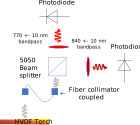
\includegraphics[width=0.8\textwidth]{\repodir/final/figures/schematics/output/PD_setup.png}
    \caption{Photodiode (PD) setup schematic. The acronyms are FCL: fiber coupled lens, BS: beam splitter, PB: bandpass filter, PD: photodiode, AMP: transimpedance amplifier, Osc.: Oscilloscope}
    \label{fig:SI_PD_setup_schematic}
\end{figure}



\begin{figure}[]
    \centering
    \includegraphics[width=0.8\textwidth]{\repodir/final/figures/setup_images/Photodiode_Setup.png}
    \caption{Image of the photodiode setup. Taken on 2023-05-24. }
    \label{fig:SI_PD_setup_image}
\end{figure}






\clearpage
\subsection{Emulsion Preparation and Delivery}

Potassium was introduced into the HVOF system by creating a potassium carbonate (K2CO3) brine and kerosene emulsion. The emulsion was delivered into the HVOF fuel flow via a tee. The tee run carried the fuel flow while the tee branch accepted emulsion through a PTFE feed line which was served by a high-pressure syringe pump. The emulsion was loaded into three syringes in the Syringe pump with the syringe outputs manifolded together. A switching valve allowed syringes to withdraw emulsion from the stirred reservoir or to infuse emulsion into the HVOF fuel line. Before, igniting the torch, the 4.8 m emulsion line was filled. At the tee, fuel flow momentum was used to mix the emulsion with the fuel flow over the 15cm distance between the tee and combustion chamber nozzle. 

Literature was reviewed for an emulsion specifically designed to work with brine – especially water-in-oil (W/O) emulsions.  Developing emulsions for use in oilfields, Mohamed et al.\cite{mohamedInfluenceSurfactantStructure2017a} investigated high salinity W/O emulsions between “formation brine” and diesel. According to these authors, “[D]iesel and kerosene are used in the oilfields because of availability.” Their formation brine included more than 221,673 mg total dissolved solids (TDS) per liter of brine (~20\% by mass).  

We noted the most stable result in \cite{mohamedInfluenceSurfactantStructure2017a} “reproduced” it using a potassium carbonate brine, kerosene, and a SPAN 80 / TWEEN 80 surfactant blend meeting their recommended Hydrophilic-lipophilic balance (HLB) of 6.8. The concentration of the surfactant was 0.5\% of the emulsion by volume - the minimum necessary found in \cite{mohamedInfluenceSurfactantStructure2017a} to obtain a stable emulsion. (Mohamed et al. measured ~5\% of liquid came out of emulsion in 100 minutes at 120 °C).  

To generate the initial brine droplets, we used a spray nozzle. Spraying to create an emulsion is a standard practice \cite{atkinsonKeroseneEmulsionHow1890} used in this work because it avoids the temperature-rise associated with higher energy processes. These spray-generated droplets were then passed through an ultrasonic process to break them up further. This continuous process also minimized temperature rise because the material exited seconds after entering the ultrasonic field. 

The emulsion preparation process is given below. 

1 . Prepare liquid components ahead of time 
  \begin{itemize}
  \item 100g supply of surfactant blend with HLB=6.8 by mixing 77g of Span 80 and 23g of Tween 80 on a magnetic stir plate 

  \item Eight aliquots of K2CO3 brine by mixing 847.7g of K2CO3 powder into 350mL of deionized water on a magnetic stirrer 

  \item Eight aliquots of prepared kerosene by mixing 5g of the surfactant blend into 106.5g of kerosene  

  \item Each Brine/Kerosene aliquot pair will produce 500mL of emulsion. 
  \end{itemize}


2. Create a pre-emulsion 

  \begin{itemize}
    
  \item Decant an aliquot of prepared kerosene into a beaker and begin stirring on a magnetic stir plate. 

  \item Pump (peristaltic)the aliquot of K2CO3 brine through a spray nozzle, producing a mist of droplets to fall into the prepared kerosene. Droplet/kerosene interfaces adsorb the surfactant to make a relatively fine pre-emulsion. 

  \end{itemize}

3. Sonicate the pre-emulsion to create the final emulsion. 

  \begin{itemize}

  \item While continuing to magnetically stir, pump the pre-emulsion through an ultrasonic continuous flow cell to further break up the dispersed brine droplets. 

  \item Batches were stored overnight and combined in magnetically stirred reservoir at the beginning of the photoionization experiment. 
  \end{itemize}

Figure \ref{fig:SI_Emulsion_Process} shows a schematic of the emulsion preparation process outlined above. 


\begin{figure}[]
\centering
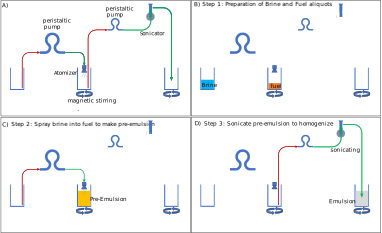
\includegraphics[width=0.8\textwidth]{\repodir/final/figures/schematics/output/Emulsion_Process.png}
\caption{Schematic of the emulsion preparation process. A) Overview of the emulsion preparation setup. B -D) Steps 1-3 of the emulsion preparation process.}
\label{fig:SI_Emulsion_Process}
\end{figure}


The emulsion recipe is given in Table \ref{tab:emulsion_parameters}. The mass of the fuel was incorrectly used as 109 g to calculate setpoints on on each day except 2023-05-24, instead of 106.5 g. The emulsion recipe on 2023-05-24 corresponds to the physical emulsion prepared on each date, and is used in the calculation of process parameters including the potassium mass fraction, equivalence ratio, and total mass flow. 


\begin{table}[h]
\centering
\begin{tabular}{|l|l|l|}
\hline
\textbf{Parameter} & \textbf{2023-04-07 to 2023-05-18} & \textbf{2023-05-24} \\
\hline
$M_{K2CO3}$ & 84.7 gram & 84.7 gram \\
$M_{fuel}$ & 109.0 gram & 106.5 gram \\
$M_{water}$ & 350.0 gram & 350.0 gram \\
$M_{span80}$ & 3.84 gram & 3.84 gram \\
$M_{tween80}$ & 1.17 gram & 1.17 gram \\
$\rho_m$ & 1.056 gram / milliliter & 1.056 gram / milliliter \\
$M_{total}$ & 548.71 gram & 546.21 gram \\
$f_{fuel}$ & 0.19865 dimensionless & 0.19498 dimensionless \\
$f_{K2CO3}$ & 0.15436 dimensionless & 0.15507 dimensionless \\
\hline
\end{tabular}
\caption{Emulsion Recipe. M = mass. $rho_m$ is the measured mass density. $M_{total}$ is the calculated total mass. $f_{fuel}$ and $f_{K2CO3}$ are the calculated mass fraction of fuel and $K_2CO_3$, respectively. The mass density ($\rho_m$) was measured by withdrawing a sample (about 10 ml) of emulsion and weighing it.  }


\label{tab:emulsion_parameters}
\end{table}
A representative picture of an emulsion batch is shown in \ref{fig:SI_Emulsion_Picture}, taken the day before the 2023-04-07 experiment. 

\begin{figure}[]
\centering
\includegraphics[width=0.8\textwidth]{\repodir/final/figures/setup_images/Emulsion_Picture_2023-04-07.png}
\caption{A picture of the potassium emulsion used on 2023-04-07. }
\label{fig:SI_Emulsion_Picture}
\end{figure}

\clearpage
\subsection{Additional Experiment Pictures}

\begin{figure}[]
\centering
\includegraphics[width=0.8\textwidth]{\repodir/final/figures/setup_images/2023-05-18_Full_Setup_Topcam_2.png}
\caption{Full setup with top camera. Taken on 2023-05-18.}
\label{fig:SI_Full_Setup_Topcam}
\end{figure}

\begin{figure}[]
\centering
\includegraphics[width=0.8\textwidth]{\repodir/final/figures/setup_images/2023-05-24_PI_Setup.png}
\caption{Full view of experiment setup. Taken on 2023-05-24.}
\label{fig:SI_Full_Setup_PI}
\end{figure}

% final/figures/setup_images/2023-05-24_Rear_View.png

\begin{figure}[]
\centering
\includegraphics[width=0.8\textwidth]{\repodir/final/figures/setup_images/2023-05-24_Rear_View.png}
\caption{Rear view of experiment setup. Taken on 2023-05-24. The optical processing setup (beam splitter, filters, and photodiode) of the PD diagnostic can be seen on the table. }
\label{fig:SI_Rear_View}
\end{figure}

\begin{figure}[]
\centering
\includegraphics[width=0.8\textwidth]{\repodir/final/figures/setup_images/2023-05-18_Top_View.jpg}
\caption{Top view of experiment setup. Taken on 2023-05-18.}
\label{fig:SI_Top_View}
\end{figure}


